\chapter{Projectile Motion}
\index{projectile motion}
A projectile is an object that, once thrown or dropped, continues to move only 
under the influence of gravity. Throwing a baseball, shooting a cannon, and 
diving off a high diving board are all examples. NASA flight planners use 
projectile motion to plan flight paths for space vehicles, such as sending 
rovers to Mars. You've already learned how to describe and model 
one-dimensional projectile motion in the Falling Bodies chapter. Now, we 
consider projectiles that also have horizontal motion, and therefore are 
moving in two dimensions. 

First, we will compare the motion of projectiles that are dropped versus 
horizontally launched from the same height. This will frame our discussion of 
the important concept of independence of motion: the vertical and horizontal 
motions of a projectile can be considered and described independent from each 
other. This will allow you to predict how far horizontally launched objects 
will travel before hitting the ground. Next, you'll learn to describe the 
motion of projectiles launched at an angle (like some heavy ground artillery). 
Finally, you'll use what you've learned to create a model of any projectile motion. 

\section{Comparing Projectiles}
This video was mentioned at the end of the kinematics chapter: \url{https://www.youtube.com/watch?v=zMF4CD7i3hg}.
From the video, we can see that the addition of horizontal motion does not effect how fast an object is acted upon by gravity. Both objects hit the ground at the same time, regardless of whether horizontal motion was added or not. This is because of a concept called \emph{independence of motion}.


\section{Independence of Motion}
\index{independence of motion}
In projectile motion, such as a ball being thrown off of a cliff, the horizontal and vertical components of motion are independent of each other. This means that horizontal motion (and forces in the horizontal direction) do not affect vertical motion (and forces in the vertical direction), and vice versa. This is because gravity only acts in the vertical direction.\footnote{This holds true for objects on sloped surfaces. Gravitational motion is just separated into components parallel and perpendicular to the slope. This will be covered in a future chapter.}

If you recall the falling bodies chapter, you know that the vertical motion of an object in free fall is described by the equations of unformly accelerated motion, with a constant acceleration of $9.8 \frac{m}{s^2}$ downward (this may simplified to $10 \frac{m}{s^2}$ for simplicity in many calculations).

In the horizontal direction, if we ignore air resistance (a common practice for elementary physics), there are no forces acting on the object. This means that the object will continue to move at a constant velocity in the horizontal direction.

Because the horizontal and vertical motions are independent of each other, we can use different equations to describe the motion in each direction.

\index{projectile motion!equations of}

%FIXME center
\begin{center}
    \begin{table}[]
    \begin{tabular}{|c|c|}
        \underline{Horizontal Motion}       & \underline{Vertical Motion}  \\
        \hline
        $\Delta x = v_{0x} t$      & $\Delta y = v_{0y} t + \frac{1}{2} (-g) t^2$  \\
        $v_x = v_{0x}$ (constant!) & $v_y = v_{0y} + (-g) t$   \\
        $a_x = 0$                & $a_y = -g$ 
    \end{tabular}
    \end{table}
\end{center}

Note that the velocity in the horizontal direction is \emph{\textbf{constant}}, while the velocity in the vertical direction is \emph{\textbf{not constant}} due to the acceleration of gravity ($9.8 \frac{m}{s^2}$ downward).

Let's take a look at some simple graphs comparing x motions and y motions, shown in Figures~\ref{fig:indep_motion_x} and \ref{fig:indep_motion_y}. Note that these are a general representation of projectile motion, and the scales or values may not be accurate.

\begin{figure}[htbp]
\centering
% --- First graph ---
\begin{minipage}{0.3\textwidth}
\centering
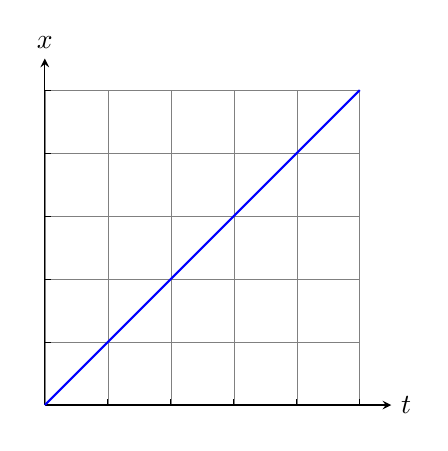
\begin{tikzpicture}[>=stealth, scale=0.8]
  \draw[help lines, step=1] (0,0) grid (5,5);
  \draw[->] (0,0) -- (5.5,0) node[right] {$t$};
  \draw[->] (0,0) -- (0,5.5) node[above] {$x$};
  \foreach \x in {1,2,3,4,5} \draw (\x,0) --++ (0,0.1);
  \foreach \y in {1,2,3,4,5} \draw (0,\y) --++ (0.1,0);
\draw[thick, blue] (0,0) -- (5,5);

\end{tikzpicture}
\caption*{x-position vs. time}
\end{minipage}
\hfill
% --- Second graph ---
\begin{minipage}{0.3\textwidth}
\centering
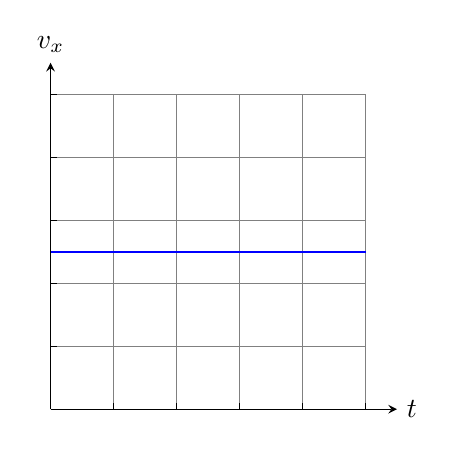
\begin{tikzpicture}[>=stealth, scale=0.8]
  \draw[help lines, step=1] (0,0) grid (5,5);
  \draw[->] (0,0) -- (5.5,0) node[right] {$t$};
  \draw[->] (0,0) -- (0,5.5) node[above] {$v_x$};
  \foreach \x in {1,2,3,4,5} \draw (\x,0) --++ (0,0.1);
  \foreach \y in {1,2,3,4,5} \draw (0,\y) --++ (0.1,0);
  \draw[thick, blue] (0,2.5) -- (5,2.5);
\end{tikzpicture}
\caption*{x-velocity vs. time}
\end{minipage}
\hfill
% --- Third graph ---
\begin{minipage}{0.3\textwidth}
\centering
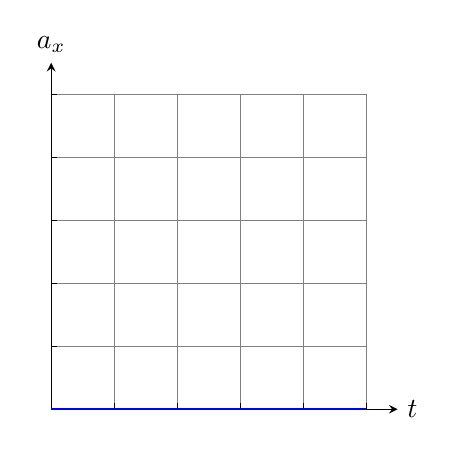
\begin{tikzpicture}[>=stealth, scale=0.8]
  \draw[help lines, step=1] (0,0) grid (5,5);
  \draw[->] (0,0) -- (5.5,0) node[right] {$t$};
  \draw[->] (0,0) -- (0,5.5) node[above] {$a_x$};
  \foreach \x in {1,2,3,4,5} \draw (\x,0) --++ (0,0.1);
  \foreach \y in {1,2,3,4,5} \draw (0,\y) --++ (0.1,0);
  \draw[thick, blue] (0,0) -- (5,0);

\end{tikzpicture}
\caption*{x-acceleration vs. time}
\end{minipage}
\label{fig:indep_motion_x}
\end{figure}

\begin{figure}[htbp]
\centering
% --- First graph ---
\begin{minipage}{0.3\textwidth}
\centering
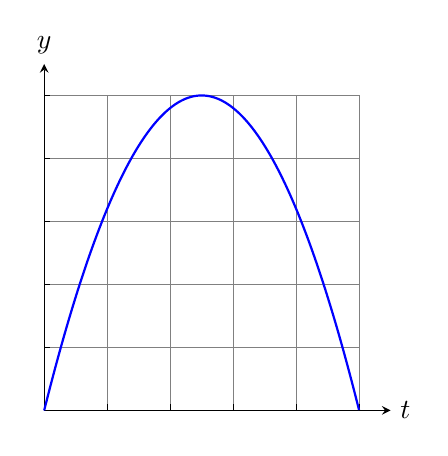
\begin{tikzpicture}[>=stealth, scale=0.8]
  \draw[help lines, step=1] (0,0) grid (5,5);
  \draw[->] (0,0) -- (5.5,0) node[right] {$t$};
  \draw[->] (0,0) -- (0,5.5) node[above] {$y$};
  \foreach \x in {1,2,3,4,5} \draw (\x,0) --++ (0,0.1);
  \foreach \y in {1,2,3,4,5} \draw (0,\y) --++ (0.1,0);
  \draw[thick, domain=0:5, samples=200, smooth, blue]
    plot (\x, {-0.8*(\x-2.5)*(\x-2.5) + 5});
\end{tikzpicture}
\caption*{y-position vs. time}
\end{minipage}
\hfill
% --- Second graph ---
\begin{minipage}{0.3\textwidth}
\centering
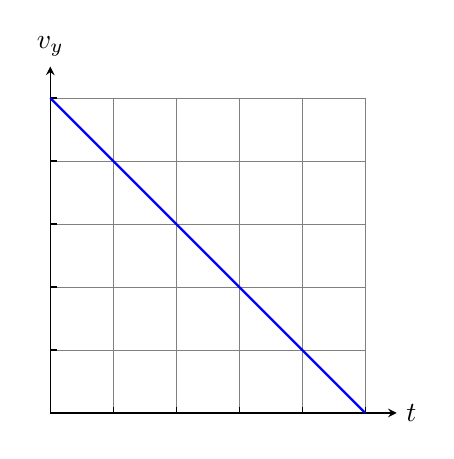
\begin{tikzpicture}[>=stealth, scale=0.8]
  \draw[help lines, step=1] (0,0) grid (5,5);
  \draw[->] (0,0) -- (5.5,0) node[right] {$t$};
  \draw[->] (0,0) -- (0,5.5) node[above] {$v_y$};
  \foreach \x in {1,2,3,4,5} \draw (\x,0) --++ (0,0.1);
  \foreach \y in {1,2,3,4,5} \draw (0,\y) --++ (0.1,0);
  \draw[thick, blue] (0,5) -- (5,0);
\end{tikzpicture}
\caption*{y-velocity vs. time}
\end{minipage}
\hfill
% --- Third graph ---
\begin{minipage}{0.3\textwidth}
\centering
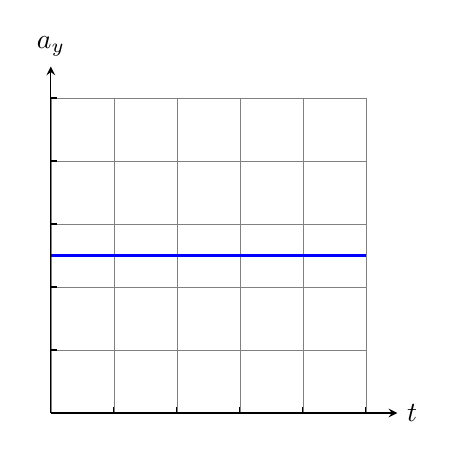
\begin{tikzpicture}[>=stealth, scale=0.8]
  \draw[help lines, step=1] (0,0) grid (5,5);
  \draw[->] (0,0) -- (5.5,0) node[right] {$t$};
  \draw[->] (0,0) -- (0,5.5) node[above] {$a_y$};
  \foreach \x in {1,2,3,4,5} \draw (\x,0) --++ (0,0.1);
  \foreach \y in {1,2,3,4,5} \draw (0,\y) --++ (0.1,0);
  \draw[thick, blue] (0,2.5) -- (5,2.5);

\end{tikzpicture}
\caption*{y-acceleration vs. time}
\end{minipage}
\label{fig:indep_motion_y}
\end{figure}


\index{horizontally launched projectiles}
\section{Horizontally-launched Projectiles}
Imagine a ball is thrown horizontally off of a cliff. The ball has an initial horizontal velocity of $20$ m/s, but no initial vertical velocity. The ball will continue to move horizontally at a constant velocity, while simultaneously accelerating downward due to gravity. The ball falls for 5 seconds before hitting the ground. We will use $-10 \frac{m}{s^2}$ for the acceleration due to gravity to make calculations easier. See figure \ref{fig:horiz_launch}.
\begin{figure}[htbp]
    \centering
    \begin{tikzpicture}
        %FIXME
        \coordinate (launchpt) at (0,5.5);
        \coordinate (cliffpt) at (0, 5);
        \coordinate (corner) at (0, 0);
        \coordinate (groundpt) at (10, 0);
    
        \filldraw (launchpt) circle [radius=.1, red] node[below] {Launch Point};
        \draw[thin] (-5, 5) --(cliffpt) -- (corner) -- (groundpt);
        \draw[->] (launchpt) -- ++(1,0) node[midway, above] {$v_{0x} = 20 \frac{m}{s}$};
    
        \draw[dashed, blue, domain=0:4.7, samples=50, thick]
            plot (\x, {5.5 - 0.25*(\x)^2});
    \end{tikzpicture}
    \caption{Diagram of a ball being thrown horizontally off of a cliff. Note: figure is not to scale.}
    \label{fig:horiz_launch}
\end{figure}

Let's calculate the change in $y$. 

The vertical motion can be described by the equation:

\[
\Delta y = v_{0y} t + \frac{1}{2} (-g) t^2
\]

Since the initial vertical velocity $v_{0y} = 0$, this simplifies to:

\[
\Delta y = \frac{1}{2} (-g) t^2
\]

Substituting in the values for $g$ and $t$:

\[
\Delta y = \frac{1}{2} (-10 \frac{m}{s^2}) (5 s)^2
\]

Calculating this gives:

\[
\Delta y = -125 m
\]

So the ball falls a vertical distance of $122.5$ m from its origin before hitting the ground.

Now let's calculate the change in $x$.
The horizontal motion can be described by the equation:

\[
\Delta x = v_{0x} t
\]

Substituting in the values for $v_{0x}$ and $t$:
\[
\Delta x = (20 \frac{\text{m}}{\text{s}}) (5 \text{s}) = 100 \text{m}
\]

\begin{Exercise}[title=Horizontally-launched Projectile, label=projectiles_horiz1]
A rock is thrown horizontally off of the edge of a cliff with an initial velocity of $8$ m/s. If the rock falls for $3$ seconds before hitting the ground, (a) how far from the base of the cliff does the rock land? (b) How high is the cliff? 

Use $-10 \frac{m}{s^2}$ for the acceleration due to gravity.
\end{Exercise}

\begin{Answer}[ref=projectiles_horiz1]
(a) To find how far from the base of the cliff the rock lands, we can use the horizontal motion equation:
\begin{align*}
    \Delta x &= v_{0x} t\\
    \Delta x &= (8 \tfrac{\text{m}}{\text{s}})(3 \text{s}) = 24 \text{m}
\end{align*}
(b) To find the height of the cliff, we can use the vertical motion equation. Since $v_{0y} = 0$, and the initial vertical position is at the top of the cliff (we can call this $y_0 = 0$), we have:

\begin{align*}
    y_f &= v_{0y} t + \frac{1}{2} (-g) t^2 \\
    y_f &= 0 + \frac{1}{2} (-10) (3)^{2} \\
    y_f &= -45 m
\end{align*}

We get a negative value for $y_f$ because the rock is falling downward from its initial position, the top of the cliff which we selected as the origin. Therefore, the height of the cliff is $45$ meters.

So the rock lands $24$ meters from the base of the cliff, and the cliff is $45$ meters high.

\end{Answer}

\subsection{Newton's Cannon and Escape Velocity}
A real world application of horizontally launched projectiles is a thought experiment known as Newton's cannon (sometimes called Newton's cannonball). Newton theorized that a cannon on the top of a mountain above Earth's atmosphere could launch a cannonball at some high velocity could do one of three things:
\begin{itemize}
    \item The cannonball would not have enough horizontal velocity, and fall back to the Earth. 
    \item The cannonball would get shot at enough velocity to be in continuous orbit around the Earth. (This is how satellites stay in orbit around the Earth!).
    \item The cannonball would get shot at such a high velocity that it would escape the Earth's gravitational pull, and fly off into space. This is known as \emph{escape velocity}. \index{escape velocity}
\end{itemize}

Take a look at this simulation of Newton's cannon: \url{https://physics.weber.edu/schroeder/software/NewtonsCannon.html}. Then, watch this video: \url{https://www.youtube.com/watch?v=ALRdYPMpqQs}.

At anywhere below $7000$ m/s, the cannonball falls back to Earth. In a range of $7,000$ m/s to $8,000$ m/s (the simulation doesn't go above $8,000$ m/s), the cannonball enters an orbit around the Earth. For Earth, the escape velocity is $\approx \,11,200$ m/s.

For any given planet, the escape velocity can be calculated using the formula:
$${\displaystyle v_{\text{e}}={\sqrt {\frac {2GM}{d}}}}$$
where $G$ is the gravitational constant, $M$ is the mass of the planet, and $d$ is the distance from the center of the planet to the object. We will cover this in more detail in the orbits chapter.

\section{Projectiles launched at an Angle}
\index{projectile motion!at an angle}
\subsection{From the Ground}

Now, let's imagine a ball is launched from the ground at at angle. 
The angle of launch influences both horizontal and vertical components of the initial velocity. 
We can use trigonometry to separate the initial velocity into its horizontal and vertical components.

\[            
v_{0x} = v_0 \cos(\theta) \qquad \qquad
v_{0y} = v_0 \sin(\theta) 
\]

In the previous section, when an object is thrown directly horizontally, $\theta = 0 ^\circ$, so $v_{0x} = v_0$. However, we now have $v_{0}$ being seperated into two components, so the $v_{0x}$ will be less than $v_0$, as $\cos(\theta)$ and $\sin(\theta)$ are always less than or equal to 1.

The vertical component of $v_0$ is the initial velocity, $v_{0y}$. This component, unlike $v_{0x}$, is constantly changing due to gravity, at a rate of $-9.8 \frac{m}{s^2}$. The peak of an object being launched at some angle is when $v_{0y}$ is equal to 0. 


\begin{center}
    \begin{tikzpicture}
        \coordinate (origin) at (0, 0);
        \coordinate (end) at (4, 3);
        \coordinate (horiz) at (4,0);
    
        % changed coords for vector visibility
        \draw[very thick, ->] (origin) -- (3.95, 2.95) node[midway, left] {$v_0$};
        \draw[very thick, ->] (origin) -- (horiz) node[midway, below] {$v_{0x} = v_{0} \cos(\theta)$};
        \draw[very thick, ->] (horiz) -- (end) node[midway, right] {$v_{0y} = v_{0} \sin(\theta)$};
    
    
        \path
            pic[draw=black, thick, angle eccentricity=1.2, angle radius=.5cm]{right angle=end--horiz--origin};
    
        \node at ($(origin)+(0.7,0.2)$) {$\mathbf{\theta}$};
        
    \end{tikzpicture}
\end{center}

For example, take a watermelon launched at $20 \frac{m}{s}$ at an angle of $30^\circ$ above the horizontal. What would the horizontal and vertical components of the initial velocity be?

Well, we can use the equations above to find out:
$$
v_{0x} = (20) \cos(30^\circ) \approx 17.32 \text{ m/s}, \qquad v_{0y} = (20) \sin(30^\circ) = 10 \text{ m/s}
$$

It is important to note that the upwards velocity and downwards velocity are equal in magnitude at any given height (given the same vertical initial and final height), but \emph{opposite in direction}, due to the symmetric nature of projectile motion.

\begin{center}
    \begin{tikzpicture}[scale=2.5]
        \coordinate (origin) at (0, 0);
        \draw[domain=0:1.6, dashed, variable=\t]
            plot ({\t},{8*\t - 5*\t*\t});
        
        \pgfmathsetmacro{\xA}{0.2}
        \pgfmathsetmacro{\yA}{8*\xA - 5*\xA*\xA} % = 1.4
        \coordinate (vA) at (\xA,\yA);
    
        \pgfmathsetmacro{\mA}{8 - 10*\xA}        % = 6
    
        \pgfmathsetmacro{\dxA}{0.05}
        \pgfmathsetmacro{\dyA}{\mA*\dxA}
    
    
        \draw[red, thick, ->]
            ($(vA)+(-\dxA,-\dyA)$) -- ($(vA)+(\dxA,\dyA)$) node[midway, right] {$v1$};
        \fill (vA) circle[radius=0.02];
        \pgfmathsetmacro{\xB}{1.4}
        \pgfmathsetmacro{\yB}{8*\xB - 5*\xB*\xB} 
        \coordinate (vB) at (\xB,\yB);
    
        \pgfmathsetmacro{\mB}{8 - 10*\xB}      
    
        \pgfmathsetmacro{\dxB}{0.05}
        \pgfmathsetmacro{\dyB}{\mB*\dxB}
    
    
        \draw[red, thick, ->]
            ($(vB)+(-\dxB,-\dyB)$) -- ($(vB)+(\dxB,\dyB)$) node[midway, right] {$v2$};
        \fill (vB) circle[radius=0.02];
    
        \node[above right] at (2.5, 1.4) {$\mathbf{v_1 = -v_2}$};
    
    \end{tikzpicture}
\end{center}
One last formula of note is the range formula, describing the horizontal range of any object launched at an angle on \emph{level ground}:
\begin{mdframed}[frametitle={Range Formula},style=important]
    \begin{equation}
        R = \frac{v_0^2 \sin(2\theta)}{g}
    \end{equation}
    where the object starts and lands at the same vertical height. 
\end{mdframed}
\index{Range}

\begin{Exercise}[title=Projectile Motion at an angle, label=projectiles_angle1]
A pumpkin is launched at $25$ m/s at an angle of $40^\circ$ above the horizontal. Find (a) the peak height of the pumpkin, and (b) the horizontal distance the pumpkin travels before hitting the ground. Use $-10 \frac{m}{s^2}$ for the acceleration due to gravity. You may assume the ground is level the entire time. 
\end{Exercise}
\begin{Answer}[ref=projectiles_angle1]
Let's first find the horizontal and vertical components of the initial velocity:
\begin{align*}
v_{0x} &= (25) \cos(40^\circ) \approx 19.15 \text{ m/s}, \\
v_{0y} &= (25) \sin(40^\circ) \approx 16.07 \text{ m/s}.
\end{align*}

(a) To find the peak height, we can use the vertical motion equations. Taking it in two steps, let's first find the time to reach the peak height, where the vertical velocity $v_y = 0$:
\begin{align*}
    v_y = v_{0y} + (-g) t \\
    0 = 16.07 - 10t \\
    t_{peak} = \frac{16.07}{10} \approx 1.607 \text{ s}
\end{align*}
Now, we can use this time to find the peak height using the vertical displacement equation:
\begin{align*}
    \Delta y &= v_{0y} t + \frac{1}{2} (-g) t^2 \\
    \Delta y &= (16.07)(1.607) + \frac{1}{2} (-10) (1.607)^2 \\
    \Delta y &\approx 12.91 \text{ m}
\end{align*}

(b) To find the total horizontal distance traveled, we first need the total time of flight. Since the motion is symmetric, the total time will be twice the time to reach the peak height:
\[
t_{total} = 2t_{peak} \approx 2(1.607) \approx 3.214 \text{ s} = 3.21 \text{ s}
\]
Since there is no horizontal acceleration, we can use the horizontal motion equation to find the horizontal distance:
\[
\Delta x = v_{0x} t_{total} \approx (19.15)(3.21) \approx 61.5 \text{ m}
\]

So, the peak height of the pumpkin is approximately \(12.91\) m, and the horizontal distance it travels before hitting the ground is approximately \(61.5\) m.
\end{Answer}

\begin{Exercise}[title=Launch Angle for Maximum Range, label=projectiles_angle2]
(a) At what angle should you launch for an object to go the furthest given a maximum launch velocity? 
(b) How can you get the same horizontal distance with two different launch angles?
\end{Exercise}
\begin{Answer}[ref=projectiles_angle2]
To maximize the horizontal distance of a projectile being launched, the vertical and horizontal components must be proportionally equal. This is only possible at a launch angle of $45^\circ$. Let's prove this mathematically.

Let the initial launch speed be $v$ and the launch angle be $\theta$. The horizontal and vertical velocity components are
\[
v_x = v \cos\theta, \qquad v_y = v \sin\theta.
\]

The vertical motion kinematics equation can be solved for: 
\[
0 = t\Big(v \sin\theta - \tfrac{1}{2} g t\Big)
\]

This has two solutions: $t = 0$ (the time at launch) and
\[
t = \frac{2 v \sin\theta}{g}.
\]

Thus, the horizontal range is
\[
R_x = v_x \cdot t = v \cos\theta \cdot \frac{2 v \sin\theta}{g}
    = \frac{v^2}{g} \sin(2\theta).
\]

The function $\sin(2\theta)$ reaches its maximum value of 1 when $2\theta = 90^\circ$, or $\theta = 45^\circ$. Therefore, the optimal launch angle for maximum horizontal distance is $45^\circ$.

The range equation above can result can result in two different values: $\theta$ and $90^\circ-\theta$. There are two ways to get a certain horizontal launch distance, one at an angle less than $45^\circ$ and one at an angle greater than $45^\circ$. For example, a projectile launched at $30^\circ$ will travel the same horizontal distance as one launched at $60^\circ$, assuming the same initial velocity. However, the projectile launched at $30^\circ$ will spend less time in the air and have a lower peak height than the one launched at $60^\circ$.
\end{Answer}

\begin{Exercise}[title=Projectile Motion at an angle, label=projectiles_angle3]
There is a target 100 meters away. I must shoot a bow at 14 meters per second. At what angle will I be able to hit my target? If I cannot hit the target, calculate the velocity neeeded to reach the target. Use $-10 \frac{m}{s^2}$ for the acceleration due to gravity. You may assume the ground is level the entire time.
\end{Exercise}

\begin{Answer}[ref=projectiles_angle3]

Using the horizontal distance equation, $R$, with $v_0 = 14$ m/s and $R = 100$ m, we have:
\begin{align*}
R&=\frac{v^2\sin(2\theta)}{g} \\ 
\sin(2\theta) &= \frac{Rg}{v^2} \\
\sin(2\theta) &= \frac{(100)(10)}{14^2} \approx 5.10
\end{align*}
Since the sine of an angle cannot be greater than 1, it is impossible to hit the target with a launch speed of 14 m/s.

Instead, we can calculate the minimum launch speed needed to hit the target at a $45^\circ$ angle, while satisfying the $100$ m requirement. Assuming the $\sin(2\theta) = 1$ for a $45^\circ$ launch angle, we can rearrange the range equation to solve for $v$:
\begin{align*}
v &= \sqrt{\frac{Rg}{\sin(2\theta)}} \\
v &= \sqrt{\frac{(100)(10)}{1}} = \sqrt{1000} \approx 31.62 \text{ m/s}
\end{align*}

So at an assumed launch angle of $45^\circ$, a minimum launch speed of approximately $31.62$ m/s is needed to hit the target 100 meters away.
\end{Answer}




% %FIXME question for finding accel on a planet - questionbank??
\subsection{From a Height Above the Ground}
Now we can imagine a ball being launched at some angle from a height above the ground. This is similar to the horizontally launched projectile, except now we have an initial vertical velocity component.

Let's say a ball is launched from a height of $50$ m at an angle of $30^\circ$ above the horizontal with an initial velocity of $20$ m/s. We can find the horizontal and vertical components of the initial velocity as follows:
%FIXME diagram


$$v_{0x} = (20) \cos(30^\circ) \approx 17.32 \text{ m/s}, \qquad v_{0y} = (20) \sin(30^\circ) = 10 \text{ m/s}.$$
The vertical motion can be described by the equation:
\[\Delta y = y_0 + v_{0y} t + \frac{1}{2} (-g) t^2 = 50+ 10t - 5t^2\]

Likewise, the horizontal motion of the projectile can be described by the equation:
\[\Delta x = v_{0x} t = 17.32t\]

To find the peak of the projectile, we can set $v_y = 0$ and solve for $t$:
\begin{align*}
    v_y &= v_{0y} + (-g) t \\
    0 &= 10 - 5t^2 \\
    t_{peak} &= \sqrt{2} \text{ s} \approx 1.414 \text{ s}
\end{align*}

Substituting this time into the vertical and horizontal equations, we can find the peak height and horizontal distance at the peak:
\[
\Delta y = 50 + 10(\sqrt{2}) - 5(\sqrt{2})^2 = 50 + 10\sqrt{2} - 10 = 40 + 10\sqrt{2} \approx 54.14 \text{ m}
\]
\[
\Delta x = 17.32(\sqrt{2}) \approx 24.49 \text{ m}
\]

And to find the total time of flight, we can set $\Delta y = 0$ and solve for $t$:
\begin{align*}
    0 &= 50 + 10t - 5t^2 \\
    0 &= -5t^2 + 10t + 50 \\
    0 &= t^2 - 2t - 10
\end{align*}

Using the quadratic formula, we find:
\begin{align*}
    t &= \frac{- \left(\right. - 2 \left.\right) \pm \sqrt{\left(\right. - 2 \left.\right)^{2} - 4 \left(\right. 1 \left.\right) \left(\right. - 10 \left.\right)}}{2 \left(\right. 1 \left.\right)} \\ 
    &= \frac{2 \pm \sqrt{4 + 40}}{2} \\
    &= \frac{2 \pm \sqrt{44}}{2} \\
    &= 1 \pm \sqrt{11} \approx 4.32 \text{ s (taking the positive root)}
\end{align*}

\section{Simulating Projectile Motion}
% python script?



% issue number 5 in questionbank
% add projectile motion questions to questionbank